\documentclass[polish,polish,a4paper]{article}
\usepackage[T1]{fontenc}
\usepackage[utf8]{inputenc}
\usepackage{pslatex}
\usepackage{setspace}
\usepackage{caption}
\usepackage{amssymb}
\usepackage{amsmath}
\usepackage{anysize}
\usepackage{graphicx}
\usepackage{hyperref}
\usepackage{float}
\usepackage[polish]{babel}
\hypersetup{
	colorlinks=true,
	linkcolor=blue,
	filecolor=magenta,      
	urlcolor=cyan,
}
\marginsize{2.5cm}{2.5cm}{2cm}{2cm}


\begin{document}
	
\begin{spacing}{1.5}
		\begin{titlepage}
		\vspace*{\fill}
		\begin{center}
			{\Large Algorytmy i struktury danych \\[0.1cm]
				Sprawozdanie z zadania w zespołach nr. 1\\[0.1cm]
				prowadząca: dr hab. inż. Małgorzata Sterna, prof PP}\\[0.7cm]
			{\huge Algorytmy sortujące\\ [0.7cm]}
			{\large autorzy:\\[0.1cm]}
			{\Large Piotr Więtczak nr indeksu 132339,\\[0.1cm] Tomasz Chudziak nr indeksu 136691}\\[0.5cm]
			\today
		\end{center}
		\vspace*{\fill}
	\end{titlepage}
	
	\section{Implementacja algorytmów sortujących}
	Do implementacji metod sortowania posłużyliśmy się językiem $ C++ $, każda metoda została napisana  w odrębnej  funkcji, która za parametry przyjmuje kolejno: wskaźnik na tablicę, rozmiar sortowanej tablicy oraz jako ostatni wartość opcjonalną “reverse” typu bool, która odpowiada za to czy tablica będzie posortowana rosnąco czy malejąco. Do mierzenia czasu poszczególnych metod użyliśmy klasy $ std::chrono::high::resolution\_clock  $ z biblioteki $ chrono $.
	\section{Badana zależność czasu obliczeń $ t[s]$ od liczby sortowanych elementów~$ n $. }
	
	\subsection{Podział metod sortowania}
	W celu zachowania przejrzystości  otrzymanych danych podzieliliśmy metody na dwie grupy, "wolne" (Insertion Sort, Selection Sort, Bubble Sort) i $ " $szybkie$ " $ (Counting Sort, Quick Sort, Merge Sort, Heap Sort). Różnice w zależności czasu obliczeń $ t[s]$ od liczby sortowanych elementów~$ n $ dla algorytmów $ " $wolnych$ " $ i $ " $szybkich$ " $ przedstawiają poniższe wykresy.\\
	
	
\begin{minipage}[H]{\textwidth}
	\centering
	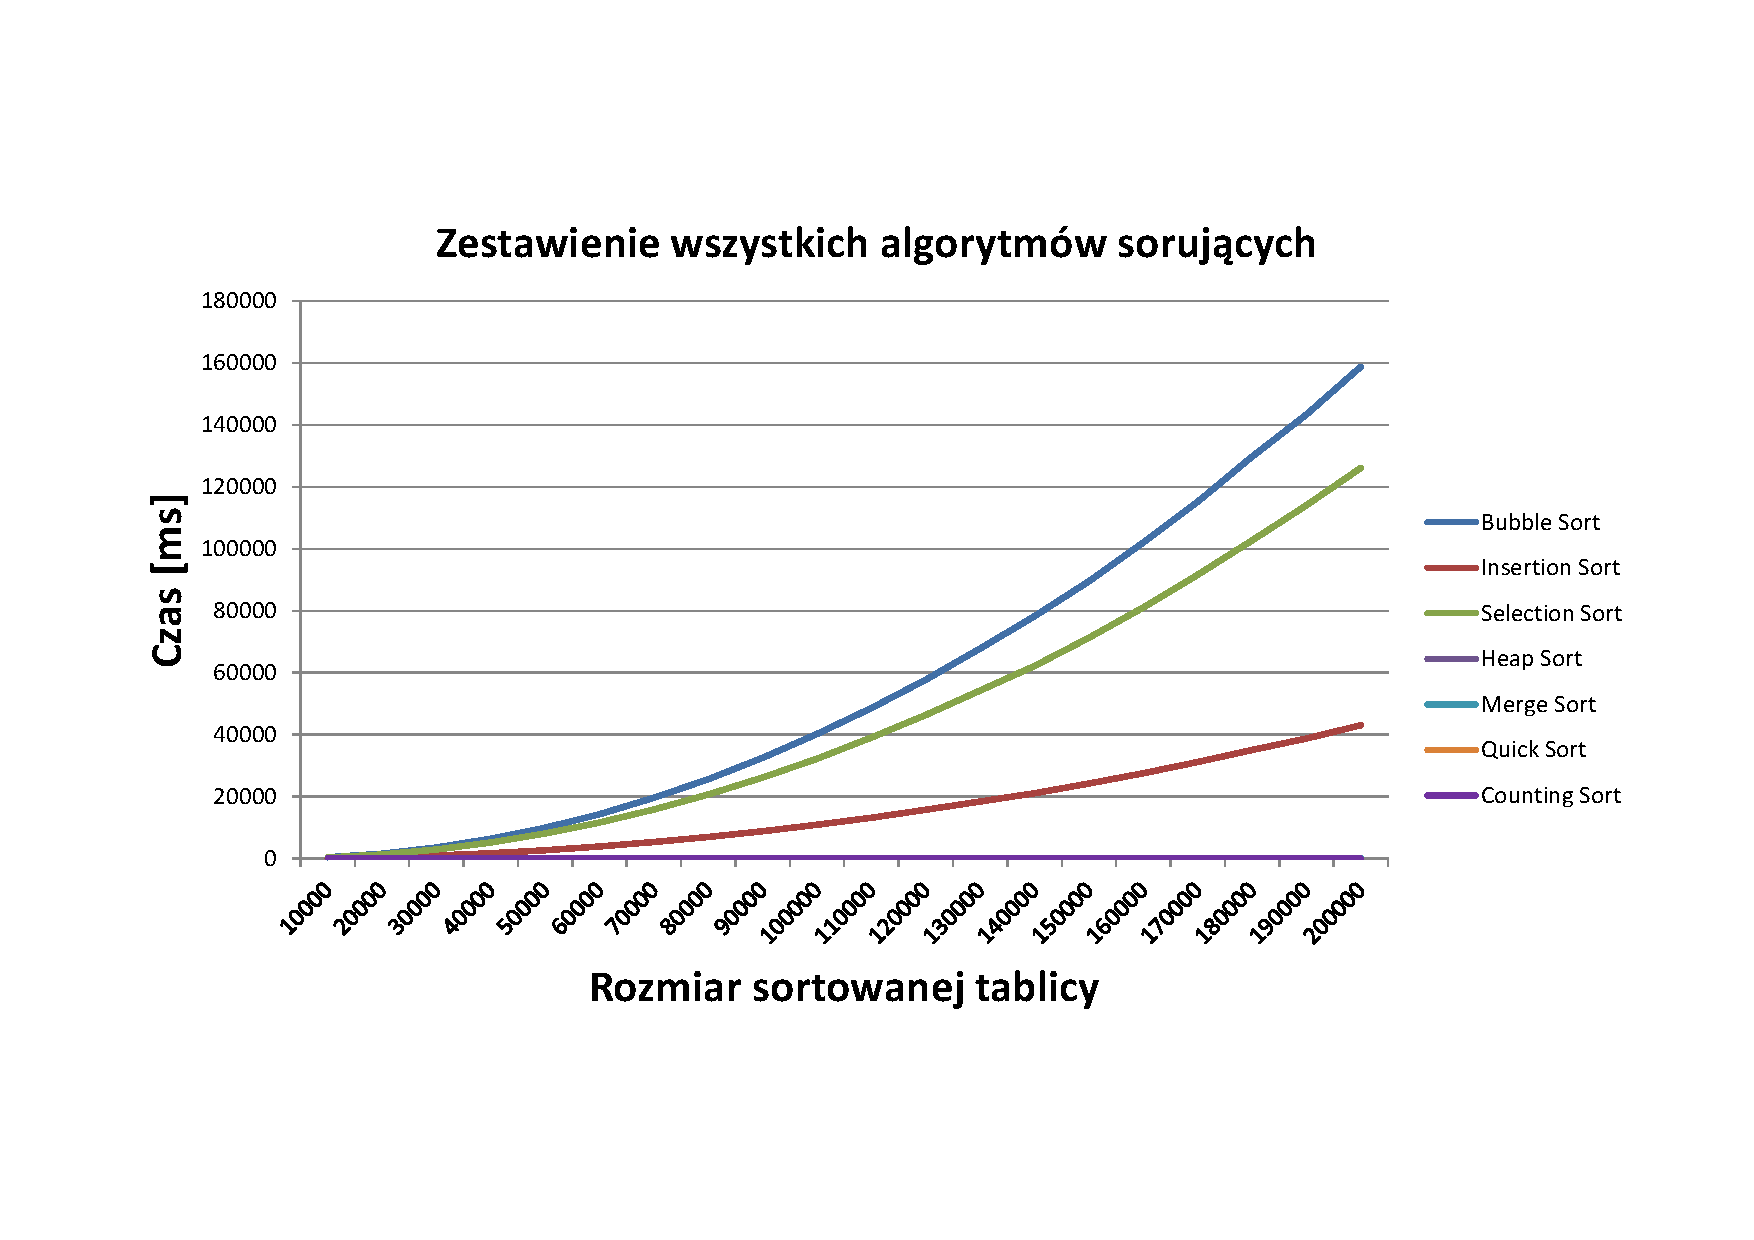
\includegraphics[scale=0.6]{zad2wsznor.pdf}
	\label{fig:2wszn}
\end{minipage}

\begin{minipage}[H]{\textwidth}
	\centering
	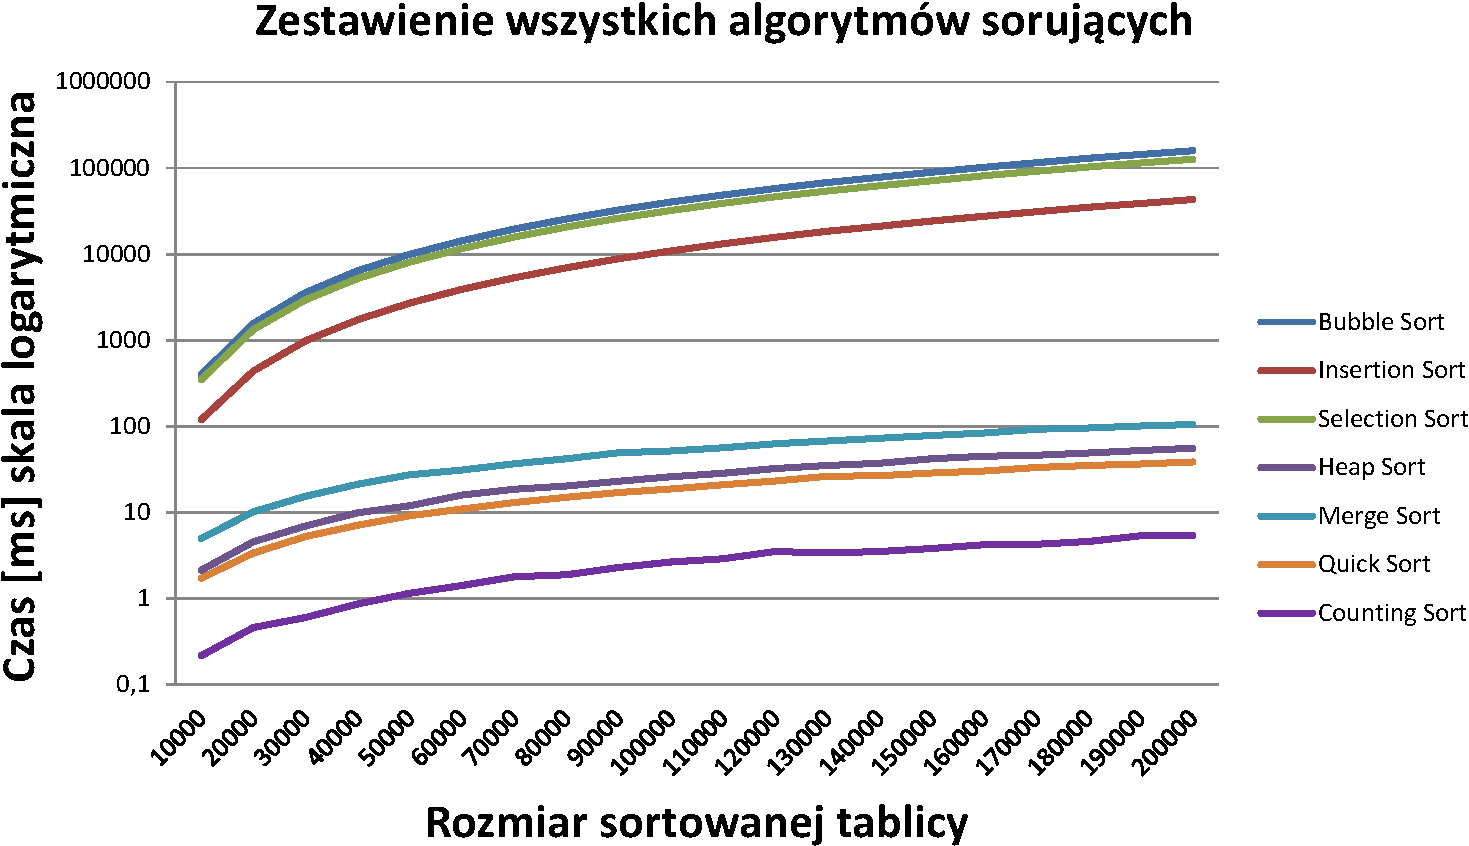
\includegraphics[scale=0.6]{zad2wszlog.pdf}
	\label{fig:2wszl}
\end{minipage}
	
	\subsection*{Wnioski do podziału metod sortowania}
	
	Jak widać na \hyperref[fig:2wszn]{wykresie} przedstawiajacym zależność czasu obliczeń od liczby sortowanych elementów, linie przedstawiające metody $ " $szybkie$ " $ zlewają się ze sobą i leżą przy samej osi OX, \hyperref[fig:2wszn]{wykres} pokazuje także jak znacząca jest różnica szybkości wykonywania sortowań między grupami. Dopiero przedstawienie danych na \hyperref[fig:2wszl]{wykresie} ze skalą logarytmiczną pozwala rozróżnić metody $"$szybkie$"$.
	
	\subsection{Metody $ "$wolne$" $}
	\subsubsection{Opis algorytmów $"$wolnych$"$}
	\subsubsection*{Insert Sort}
	Zalety:
	\begin{itemize}
		\item działa w miejscu
		\item stabilny 
	\end{itemize}
	Wady:
	\begin{itemize}
		\item wolniejszy od metod $ " $szybkich$ " $
		\item mało wydajne dla dużej ilości elementów do posortowania
	\end{itemize}
	Inne cechy:
	\begin{itemize}
		\item zachowanie naturalne
	\end{itemize}
	
				\subsubsection*{Tabela przedstawiająca złożoność obliczeniową dla przypadków optymistycznego, średniego i pesymistycznego} 
	
	\begin{figure}[H]
		\begin{equation*}
		\begin{array}{l|c|c|c|}

		&$złożoność obliczeniowa$&$złożoność obliczeniowa$&$złożoność obliczeniowa$\\
		&$dla przypadku$&$dla przypadku$&$dla przypadku$\\
		&$optymistycznego$&$średniego$&$pesymistycznego$\\
		\hline
		$Insert Sort$&O(n^2)&O(n^2)&O(n^2)\\
		\hline
		\end{array}
		\end{equation*}
		\captionof{table}{Tablica złożoności obliczeniowej dla metody Insert Sort}
	\end{figure}
		
		\subsubsection*{Selection Sort}
	Zalety:
	\begin{itemize}
		\item działa w miejscu
		\item stabilny 
	\end{itemize}
	Wady:
	\begin{itemize}
		\item wolniejszy od metod $ " $szybkich$ " $
		\item mało wydajne dla dużej ilości elementów do posortowania
	\end{itemize}
	Inne cechy:
	\begin{itemize}
		\item zachowanie naturalne
	\end{itemize}
	
				\subsubsection*{Tabela przedstawiająca złożoność obliczeniową dla przypadków optymistycznego, średniego i pesymistycznego} 
	\begin{figure}[H]

		\begin{equation*}
		\begin{array}{l|c|c|c|}

		&$złożoność obliczeniowa$&$złożoność obliczeniowa$&$złożoność obliczeniowa$\\
		&$dla przypadku$&$dla przypadku$&$dla przypadku$\\
		&$optymistycznego$&$średniego$&$pesymistycznego$\\
		\hline
		$Selection Sort$&O(n^2)&O(n^2)&O(n^2)\\
		\hline
		\end{array}
		\end{equation*}
		\captionof{table}{Tablica złożoności obliczeniowej dla metody Selection Sort}
	\end{figure}
	
	
			\subsubsection*{Bubble Sort}
	Zalety:
	\begin{itemize}
		\item działa w miejscu
		\item stabilny 
	\end{itemize}
	Wady:
	\begin{itemize}
		\item wolniejszy od metod $ " $szybkich$ " $
		\item mało wydajne dla dużej ilości elementów do posortowania
	\end{itemize}
	Inne cechy:
	\begin{itemize}
		\item zachowanie naturalne
	\end{itemize}
	
	
	\subsubsection*{Tabela przedstawiająca złożoność obliczeniową dla przypadków optymistycznego, średniego i pesymistycznego} 
	
	\begin{figure}[H]
			\begin{equation*}
		\begin{array}{l|c|c|c|}

		&$złożoność obliczeniowa$&$złożoność obliczeniowa$&$złożoność obliczeniowa$\\
		&$dla przypadku$&$dla przypadku$&$dla przypadku$\\
		&$optymistycznego$&$średniego$&$pesymistycznego$\\
		\hline
		$Bubble Sort$&O(n^2)&O(n^2)&O(n^2)\\
		\hline
		\end{array}
		\end{equation*}
		\captionof{table}{Tablica złożoności obliczeniowej dla metody Bubble Sort}
	\end{figure}

	\subsubsection*{Tabela ilustrująca zależności czasu sortowania od ilości elementów dla metod $"$wolnych$"$, zakres liczb $ [1,n] $.}
	
	\begin{figure}[H]
			\begin{equation*}
		\begin{array}{l|c|c|c|}

		$Liczba elementów$&$Insertion Sort$&$Selection Sort$&$Bubble Sort$\\
		\hline
		\end{array}
		\end{equation*}
		\captionof{table}{Wyniki badań zależności czasu od iloci elementów dla metod $"$wolnych$"$}
	\end{figure}
	
	\subsubsection*{Wykres ilustrujący zależności czasu sortowania od ilości elementów dla metod $"$wolnych$"$, zakres liczb $ [1,n] $.}
	
	\begin{minipage}[H]{\textwidth}
		\begin{center}
					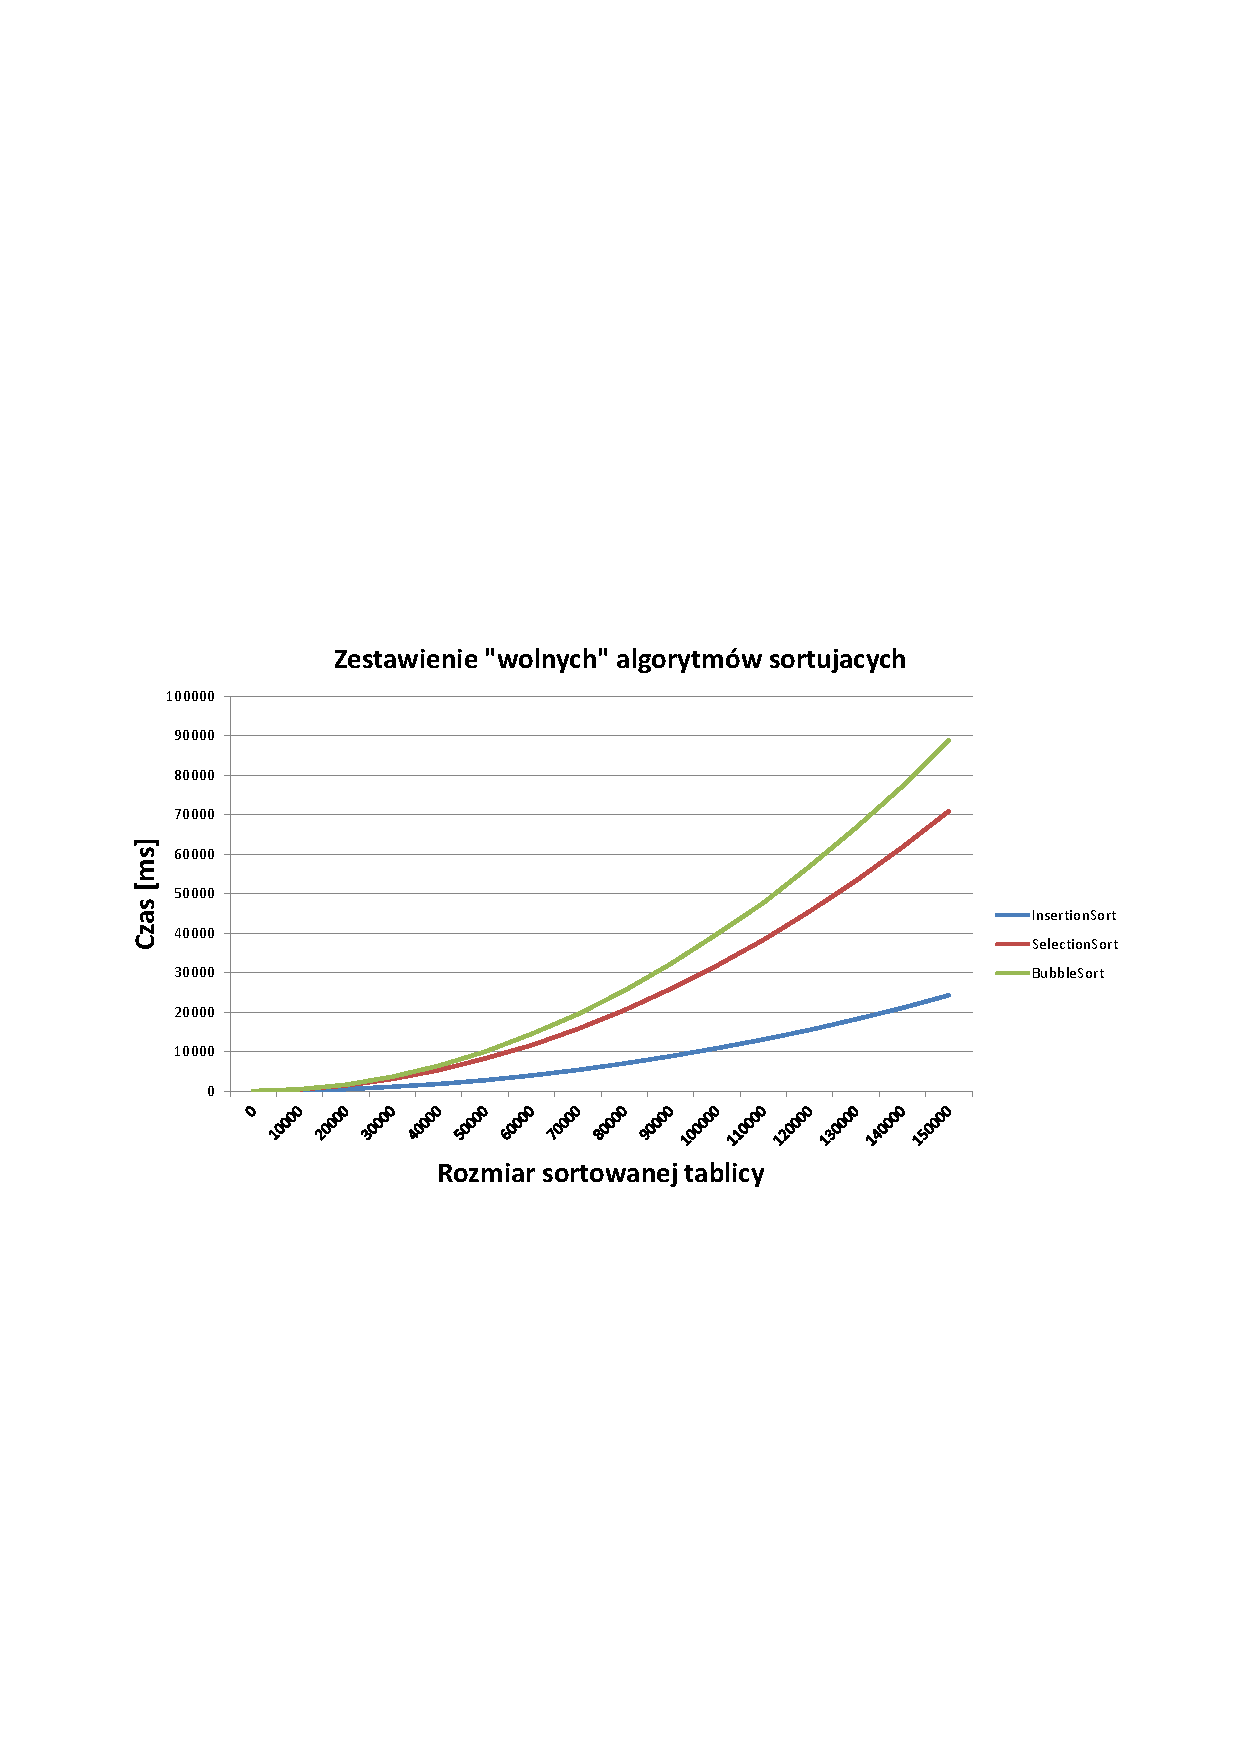
\includegraphics[scale=0.85]{zad2wolne.pdf}
					\label{fig:zad2wolne}
		\end{center}
	\end{minipage}

\subsubsection{Wnioski do metod $"$szybkich$"$}
	
	\subsection{Metody $"$szybkie$"$}

	\subsubsection{Opis algorytmów $"$szybkich$"$}

		\subsubsection*{Quick Sort}
	Zalety:
	\begin{itemize}
		\item działa w miejscu
		\item stabilny 
	\end{itemize}
	Wady:
	\begin{itemize}
		\item 
	\end{itemize}
	Inne cechy:
	\begin{itemize}
		\item zachowanie nie naturalne
		\item korzysta z metody $"$dziel i rządź$"$
	\end{itemize}
	
	\subsubsection*{Tabela przedstawiająca złożoność obliczeniową dla przypadków optymistycznego, średniego i pesymistycznego} 
	\begin{figure}[H]
		
		\begin{equation*}
		\begin{array}{l|c|c|c|}

		&$złożoność obliczeniowa$&$złożoność obliczeniowa$&$złożoność obliczeniowa$\\
		&$dla przypadku$&$dla przypadku$&$dla przypadku$\\
		&$optymistycznego$&$średniego$&$pesymistycznego$\\
		\hline
		$Quick Sort$&O(n\log_{2}(n))&O(n\log_{2}(n))&O(n^2)\\
		\hline
		\end{array}
		\end{equation*}
		\captionof{table}{Tablica złożoności obliczeniowej dla metody Quick Sort}
	\end{figure}
	
			\subsubsection*{Merge Sort}
	Zalety:
	\begin{itemize}
		\item algorytm asymptotycznie optymalny
	\end{itemize}
	Wady:
	\begin{itemize}
		\item nie działa w miejscu
		\item wrażliwy na dane wejściowe
	\end{itemize}
	Inne cechy:
	\begin{itemize}
		\item korzysta z metody $"$dziel i rządź$"$
	\end{itemize}
	
	\subsubsection*{Tabela przedstawiająca złożoność obliczeniową dla przypadków optymistycznego, średniego i pesymistycznego} 
	\begin{figure}[H]
		
		\begin{equation*}
		\begin{array}{l|c|c|c|}

		&$złożoność obliczeniowa$&$złożoność obliczeniowa$&$złożoność obliczeniowa$\\
		&$dla przypadku$&$dla przypadku$&$dla przypadku$\\
		&$optymistycznego$&$średniego$&$pesymistycznego$\\
		\hline
		$Merge Sort$&O(n\log_{2}(n))&O(n\log_{2}(n))&O(n^2)\\
		\hline
		\end{array}
		\end{equation*}
		\captionof{table}{Tablica złożoności obliczeniowej dla metody Merge Sort}
	\end{figure}
	
			\subsubsection*{Heap Sort}
Zalety:
\begin{itemize}
	\item działa w miejscu
\end{itemize}
Wady:
\begin{itemize}
	\item wrażliwy na dane wejściowe
\end{itemize}
Inne cechy:
\begin{itemize}
	\item zachowanie nienaturalne
	\item korzysta ze stogów
\end{itemize}

\subsubsection*{Tabela przedstawiająca złożoność obliczeniową dla przypadków optymistycznego, średniego i pesymistycznego} 
\begin{figure}[H]
	
	\begin{equation*}
	\begin{array}{l|c|c|c|}

	&$złożoność obliczeniowa$&$złożoność obliczeniowa$&$złożoność obliczeniowa$\\
	&$dla przypadku$&$dla przypadku$&$dla przypadku$\\
	&$optymistycznego$&$średniego$&$pesymistycznego$\\
	\hline
	$Heap Sort$&O(n)&kek&O(n\log_{2}(n))\\
	\hline
	\end{array}
	\end{equation*}
	\captionof{table}{Tablica złożoności obliczeniowej dla metody Heap Sort}
\end{figure}

			\subsubsection*{Counting Sort}
Zalety:
\begin{itemize}
	\item 
\end{itemize}
Wady:
\begin{itemize}
	\item nie działa w miejscu
	\item ograniczony ze względu na zakres sortowanych liczb
	\item mało wydajny dla danych z dużego przedziału
\end{itemize}
Inne cechy:
\begin{itemize}
	\item 
\end{itemize}

\subsubsection*{Tabela przedstawiająca złożoność obliczeniową dla przypadków optymistycznego, średniego i pesymistycznego} 
\begin{figure}[H]
	
	\begin{equation*}
	\begin{array}{l|c|c|c|}

	&$złożoność obliczeniowa$&$złożoność obliczeniowa$&$złożoność obliczeniowa$\\
	&$dla przypadku$&$dla przypadku$&$dla przypadku$\\
	&$optymistycznego$&$średniego$&$pesymistycznego$\\
	\hline
	$Counting Sort$&O(n)&O(n)&O(n)\\
	\hline
	\end{array}
	\end{equation*}
	\captionof{table}{Tablica złożoności obliczeniowej dla metody Counting Sort}
\end{figure}

	\subsubsection*{Tabela ilustrująca zależności czasu sortowania od ilości elementów dla metod $"$szybkich$"$, zakres liczb $ [1,n] $.}

\begin{figure}[H]
	\begin{equation*}
	\begin{array}{l|c|c|c|c|}
	
	$Liczba elementów$&$Quick Sort$&$Merge Sort$&$Heap Sort$&$Counting Sort$\\
	\hline
	\end{array}
	\end{equation*}
	\captionof{table}{Wyniki badań zależności czasu od iloci elementów dla metod $"$szybkich$"$}
\end{figure}

\subsubsection*{Wykres ilustrujący zależności czasu sortowania od ilości elementów dla metod $"$szybkich$"$, zakres liczb $ [1,n] $.}

	\begin{minipage}[H]{\textwidth}
	\begin{center}
		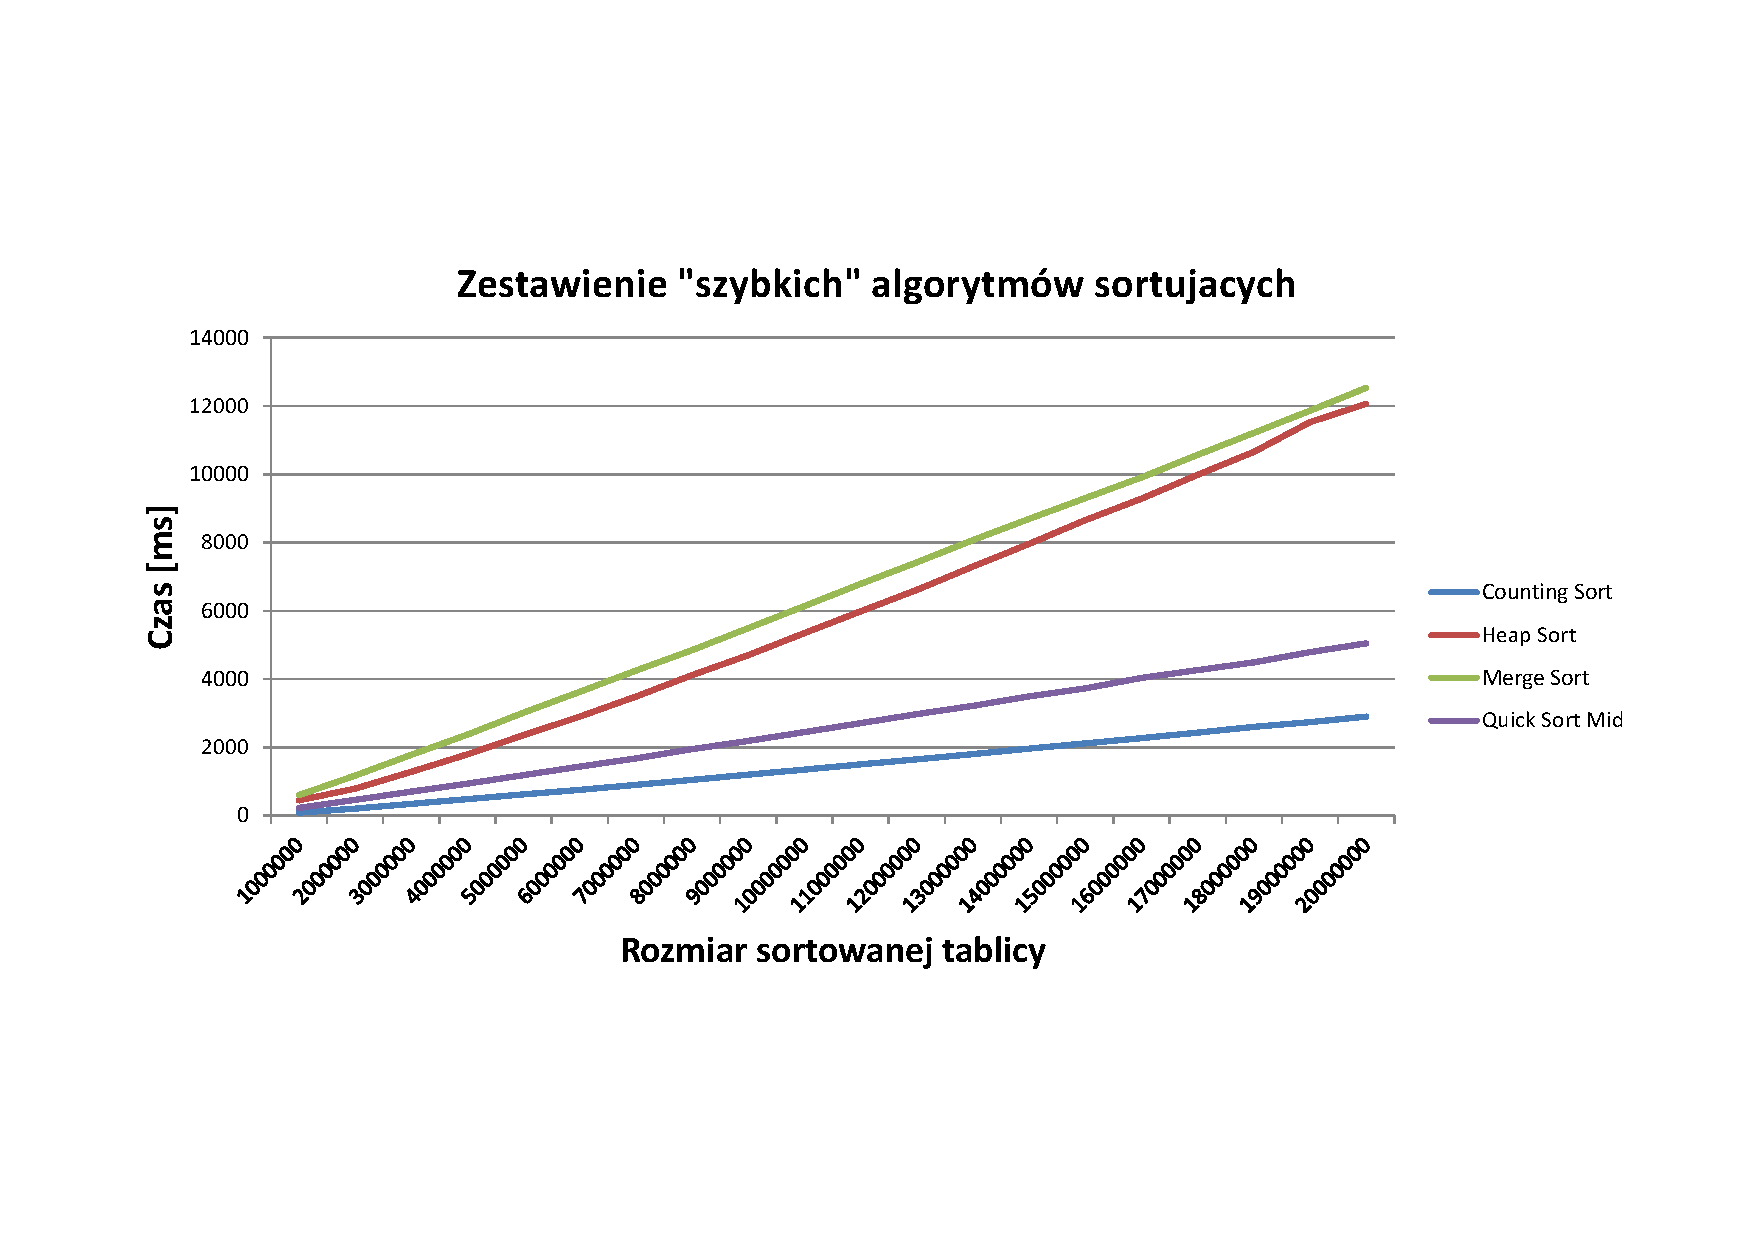
\includegraphics[scale=0.6]{zad2szybkie.pdf}
		\label{fig:zad2szybkie}
	\end{center}
\end{minipage}

\subsubsection{Wnioski do metod $"$szybkich$"$}


\subsection{Wnioski do podziału metod sortowania}

\section{Badanie zależności czasu $t$ od liczby sortowanych elementów $n$, przy rozkładach losowych i rosnących, dla metod Quick Sort z podziałem wg: skrajnego i środowego elementu, oraz dla metody Insert Sort}

W dalszej części sprawozdania algorytm Quick Sort z podziałem według środkowego elementu będziemy nazywać Quick Sort Mid, a z podziałem według skrajnego elementu Qick Sort Right.


	\subsubsection*{Tabela ilustrująca zależności czasu sortowania od ilości elementów dla metod Quick Sort Mid, Quick Sort Right, Insertion Sort, dla rozkładów losowego i rosnącego.}


\begin{figure}[H]
	\begin{equation*}
	\begin{array}{l|c|c|c|c|c|c|}
	
	&$Insert Sort$&$Quick Sort Right$&$Quick Sort Mid$&$Insert Sort$&$Quick Sort Right$&$Quick Sort Mid$\\
	$L. ele.$&$roz. losowy$&$roz. losowy$&$roz. losowy$&$roz.rosnący$&$roz. rosnący$&$roz. rosnący$\\
	\hline
	\end{array}
	\end{equation*}
	\captionof{table}{Wyniki badań zależności czasu od ilości elementów dla metod Quick Sort Mid, Quick Sort Right, Insertion Sort, dla rozkładów losowego i rosnącego.}
\end{figure}

\subsection{Rozkład losowy}

\subsubsection*{Wykresy ilustrujące zależności czasu sortowania od ilości elementów dla metod Quick Sort Mid, Quick Sort Right, Insertion Sort, dla rozkładu losowego.}

\begin{minipage}[H]{\textwidth}
	\begin{center}
		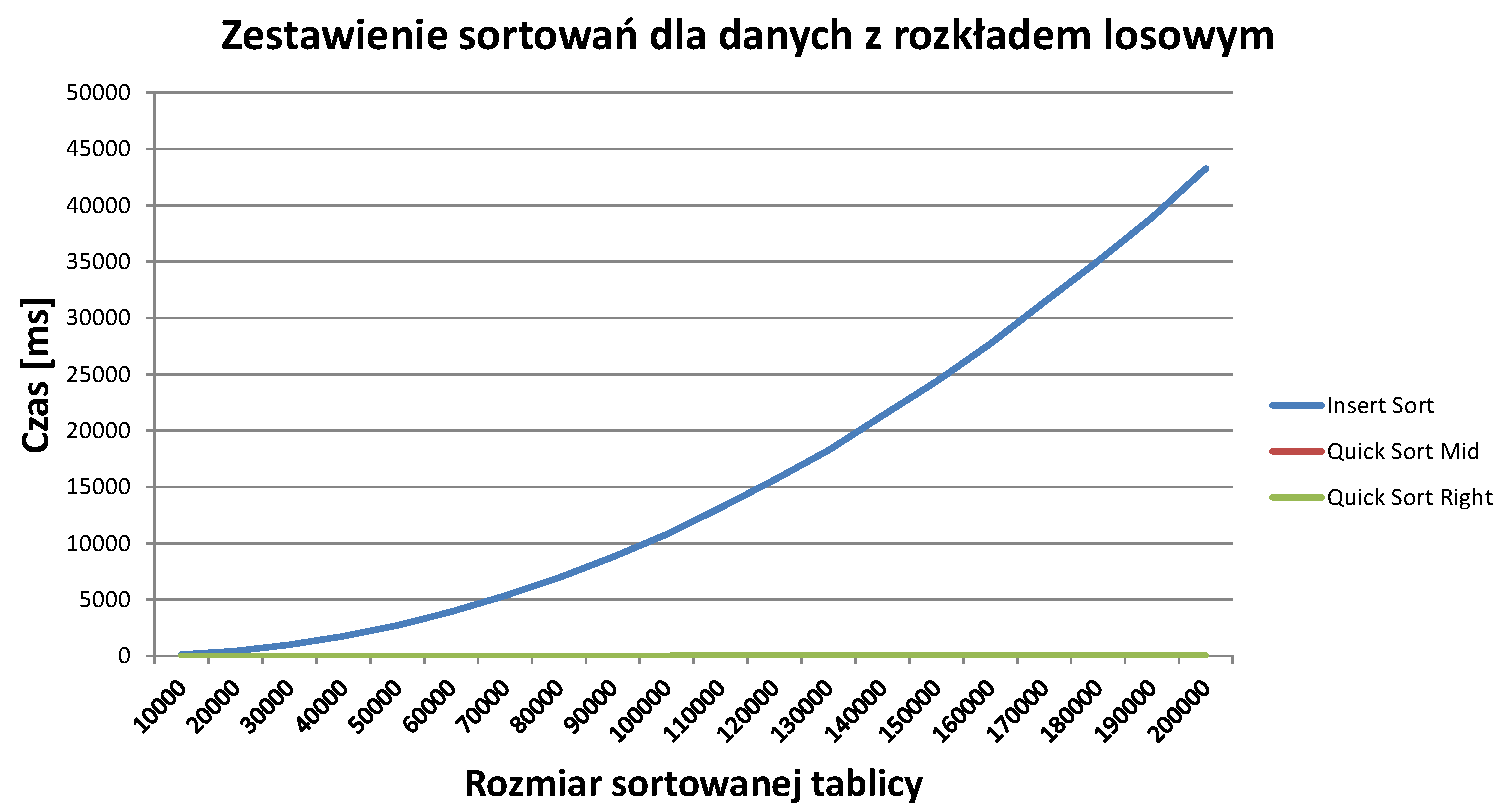
\includegraphics[scale=0.6]{zad3losowynorm.pdf}
		\label{fig:zad3losn}
	\end{center}
\end{minipage}

\begin{minipage}[H]{\textwidth}
	\begin{center}
		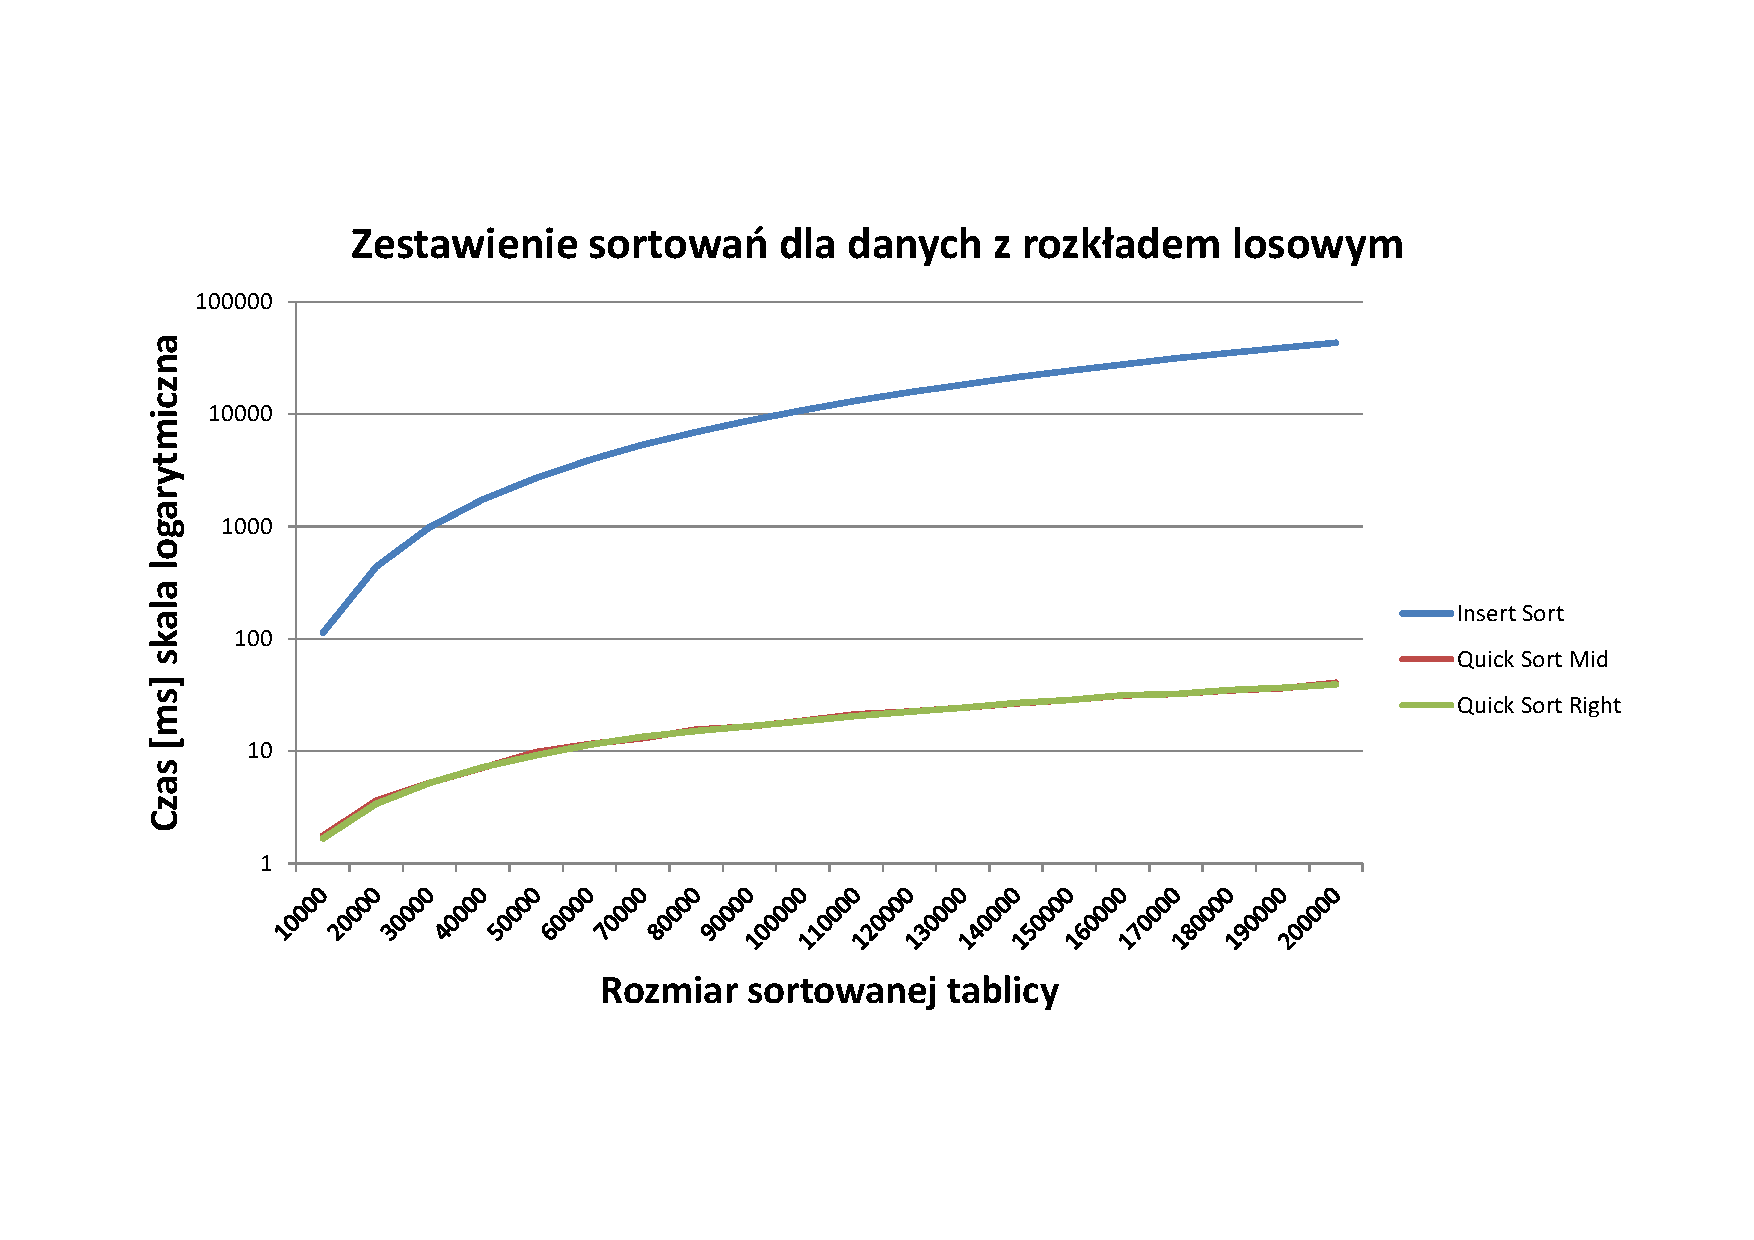
\includegraphics[scale=0.55]{zad3losowylog.pdf}
		\label{fig:zad3loslog}
	\end{center}
\end{minipage}

\subsubsection{Wnioski do rozkładu losowego}

\subsection{Rozkład rosnący}

\subsubsection*{Wykresy ilustrujące zależności czasu sortowania od ilości elementów dla metod Quick Sort Mid, Quick Sort Right, Insertion Sort, dla rozkładu rosnącego.}
	

\begin{minipage}[H]{\textwidth}
	\begin{center}
		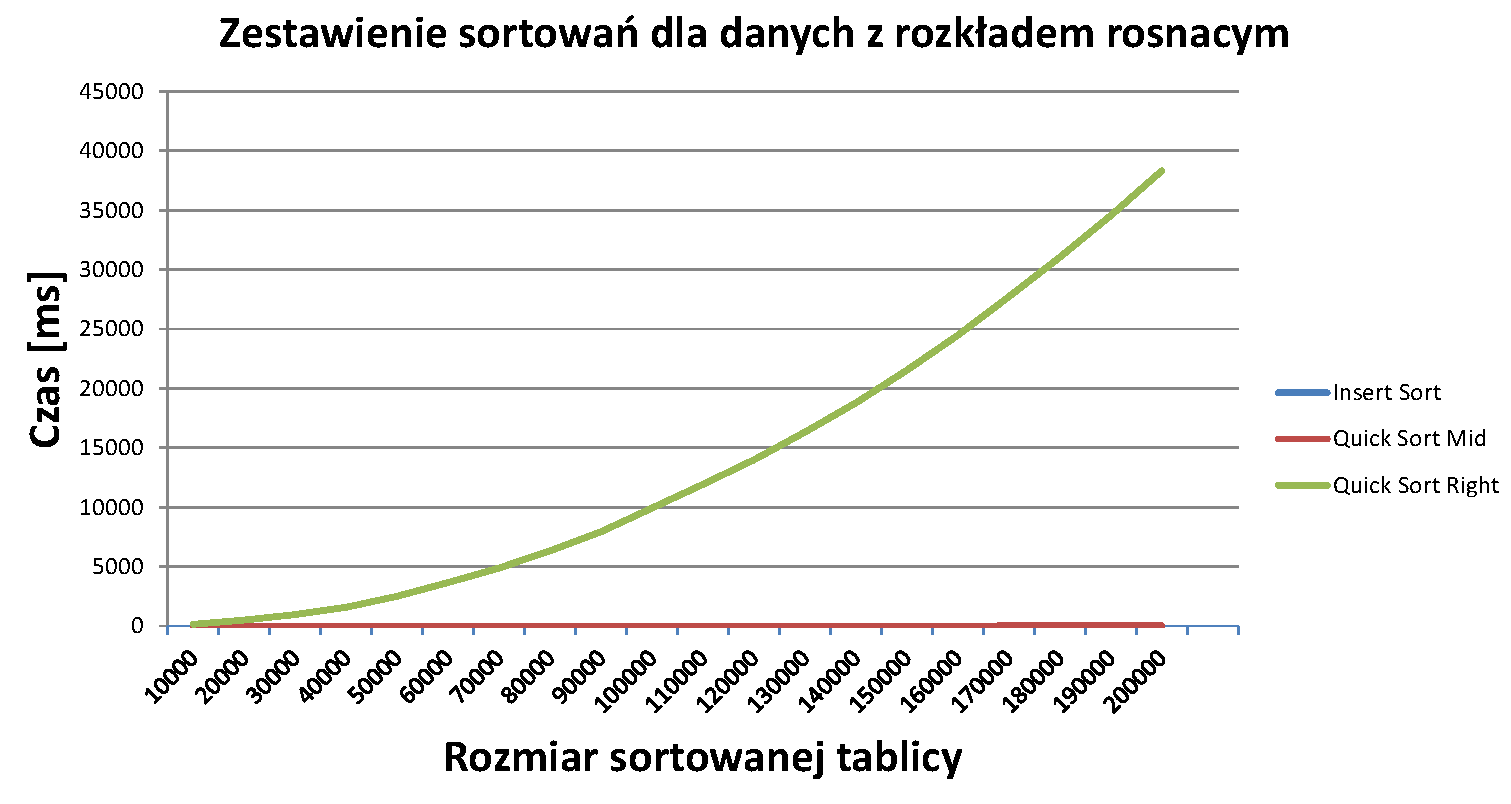
\includegraphics[scale=0.6]{zad3rosnacynorm.pdf}
		\label{fig:zad3rosn}
	\end{center}
\end{minipage}

\begin{minipage}[H]{\textwidth}
	\begin{center}
		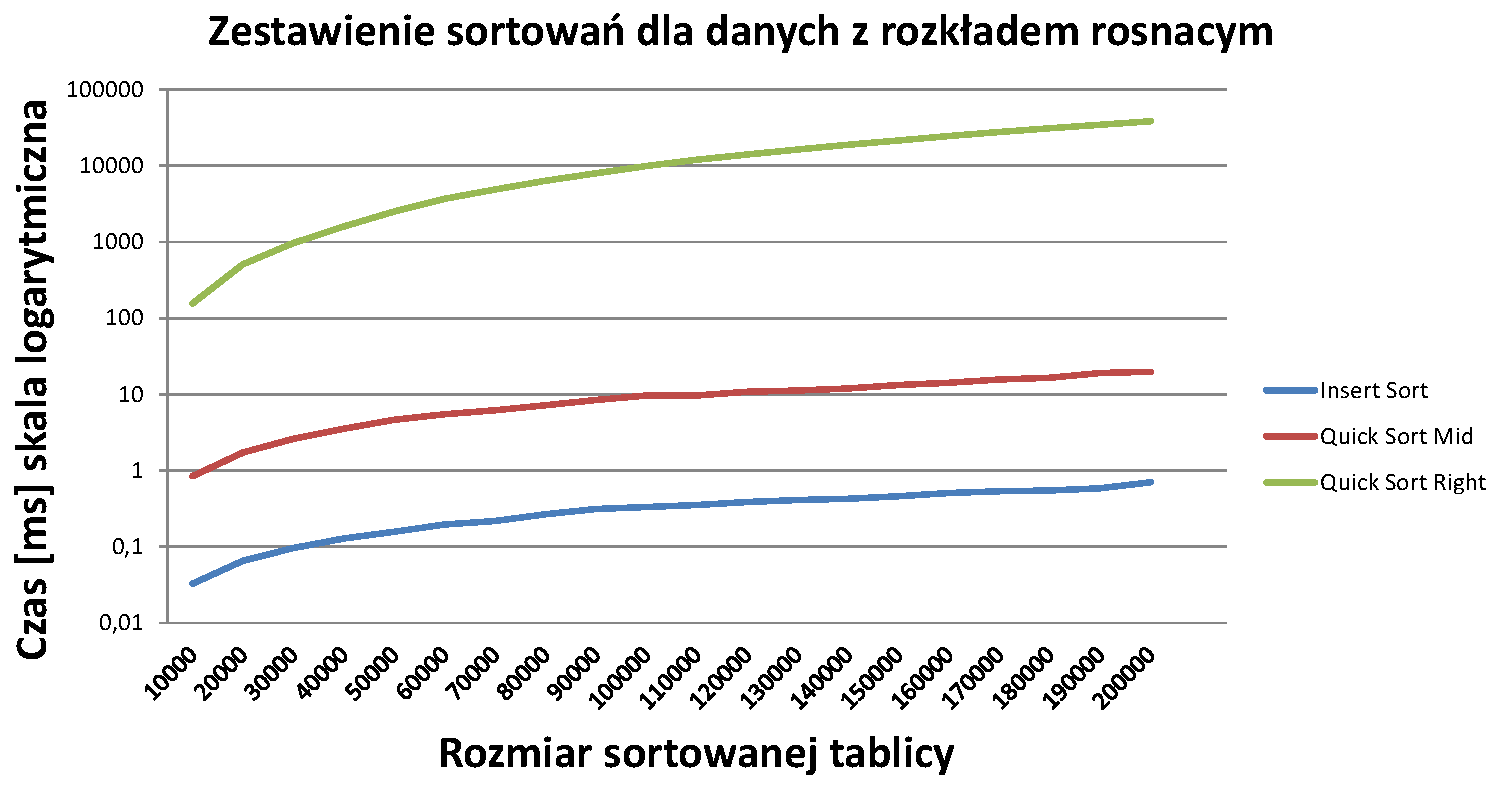
\includegraphics[scale=0.6]{zad3rosnacylog.pdf}
		\label{fig:zad3roslog}
	\end{center}
\end{minipage}


\subsubsection{Wnioski do rozkładu rosnącego}

\subsection{Wnioski do zależności czasu $t$ od liczby sortowanych elementów $n$, przy rozkładach losowych i rosnących, dla metod Quick Sort z podziałem wg: skrajnego i środowego elementu, oraz dla metody Insert Sort}

\section{Badanie zależności czasu obliczeń $t$ od liczby sortowanych elementów $n$ dla metod Counting Sort, Quick Sort, przy rozkaładzie losowym, gdy wartości elementów mieszczą się w przedziałach  $ [1;0,01n] $,$ [1;100n] $. }

\subsection{Przedział $[1;0,01n]$}

\subsubsection*{Wykres ilustrujący zależność czasu obliczeń od ilości elementów dla metod Counting Sort i  Quick Sort, dla rozkładu losowego w przedziale $[1;0,01n]$.}
	
	\begin{minipage}[H]{\textwidth}
		\begin{center}
			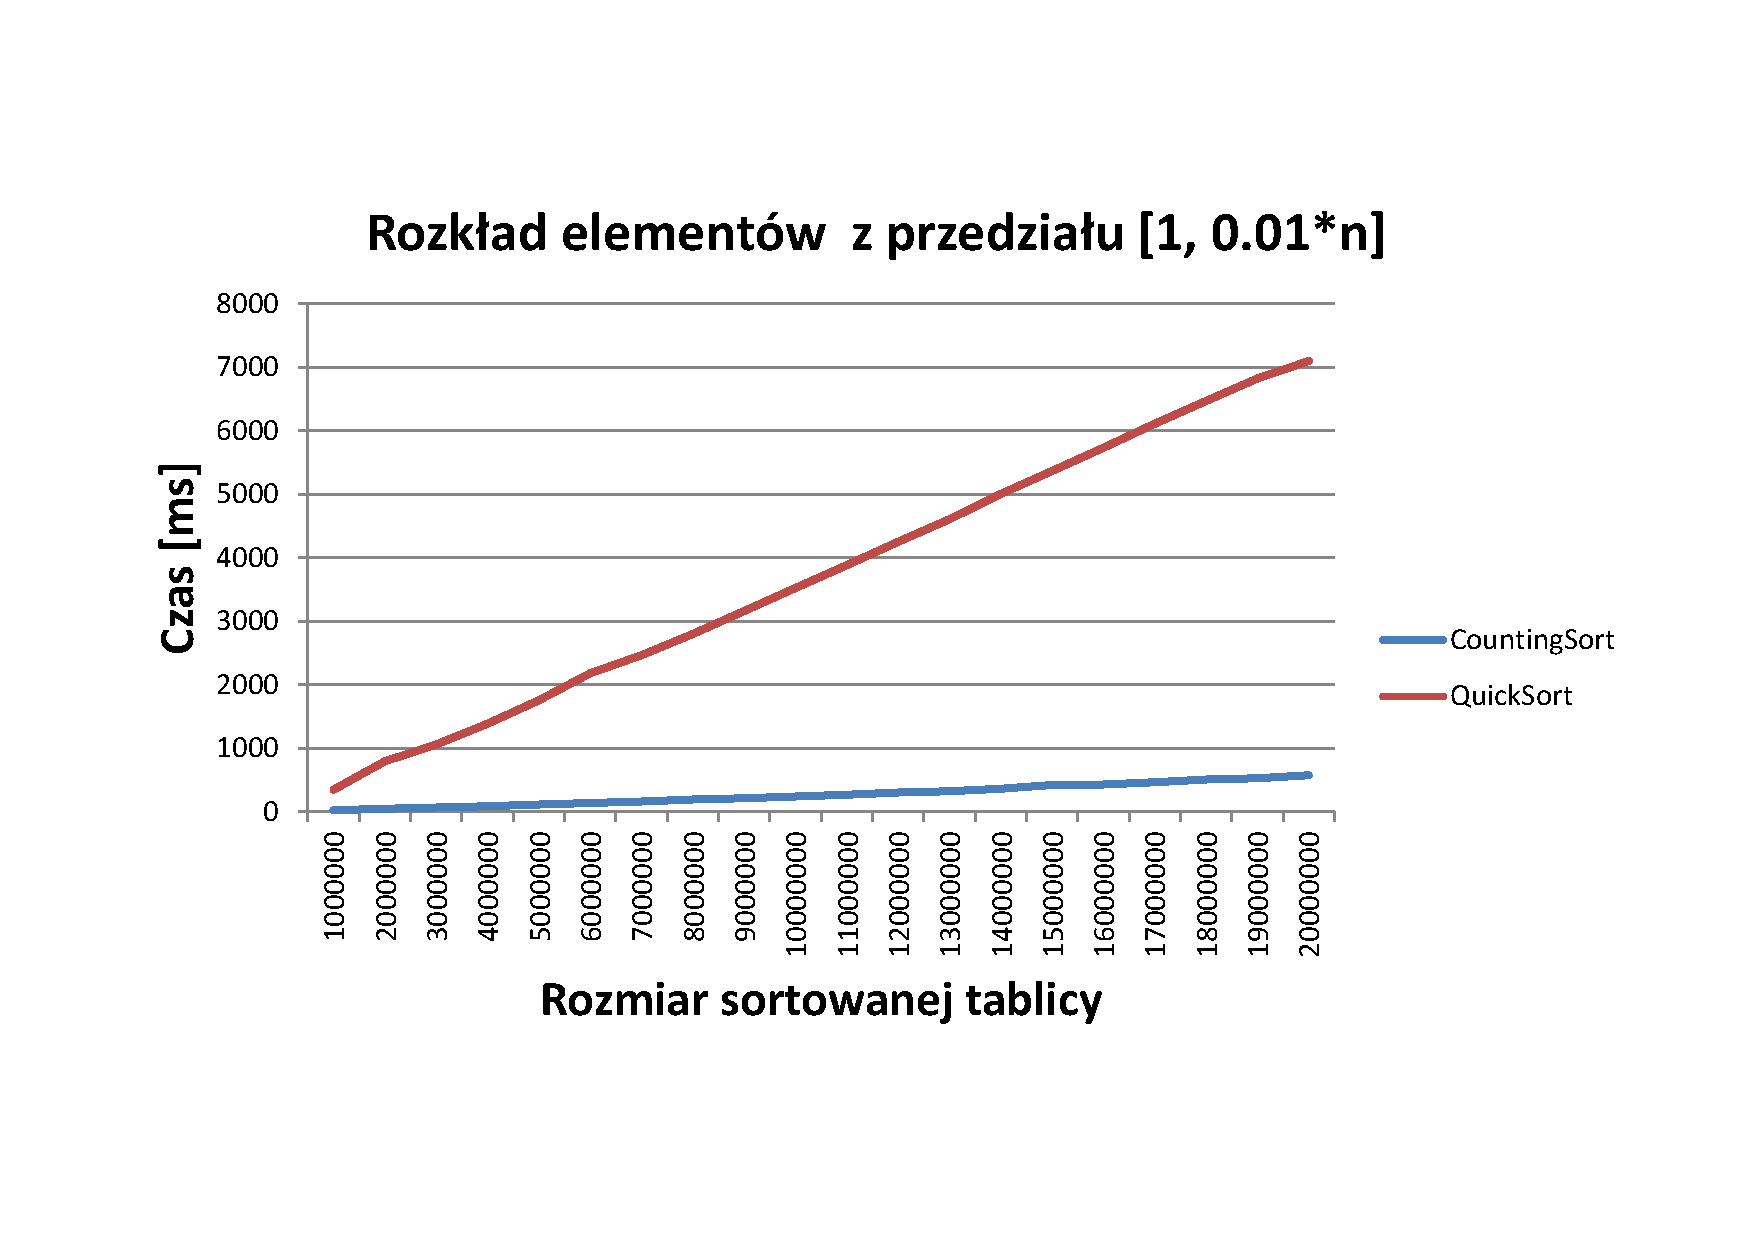
\includegraphics[scale=0.6]{zad4001n.pdf}
			\label{fig:zad4001n}
		\end{center}
	\end{minipage}

\subsubsection*{Zrzut ekranu sekcji Diagnostic Tools programu Visual Studio 2015 prezentujący, zużycie pamięci i procesora w trakcie sortowania algorytmami Counting Sort i  Quick Sort, dla rozkładu losowego w przedziale $[1;0,01n]$.}

	\begin{minipage}[H]{\textwidth}
	\begin{center}
		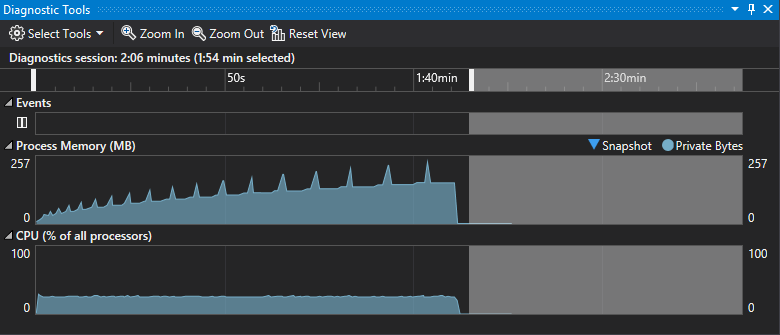
\includegraphics[scale=0.85]{zad4pamiec001n.png}
		\label{fig:zad4pamiec001n}
	\end{center}
	\end{minipage}

\subsubsection{Wnioski do przedziału $[1;100n]$}

\subsection{Przedział $[1;100n]$}

\subsubsection*{Wykres ilustrujący zależność czasu obliczeń od ilości elementów dla metod Counting Sort i  Quick Sort, dla rozkładu losowego w przedziale $[1;100n]$.}

\begin{minipage}[H]{\textwidth}
	\begin{center}
		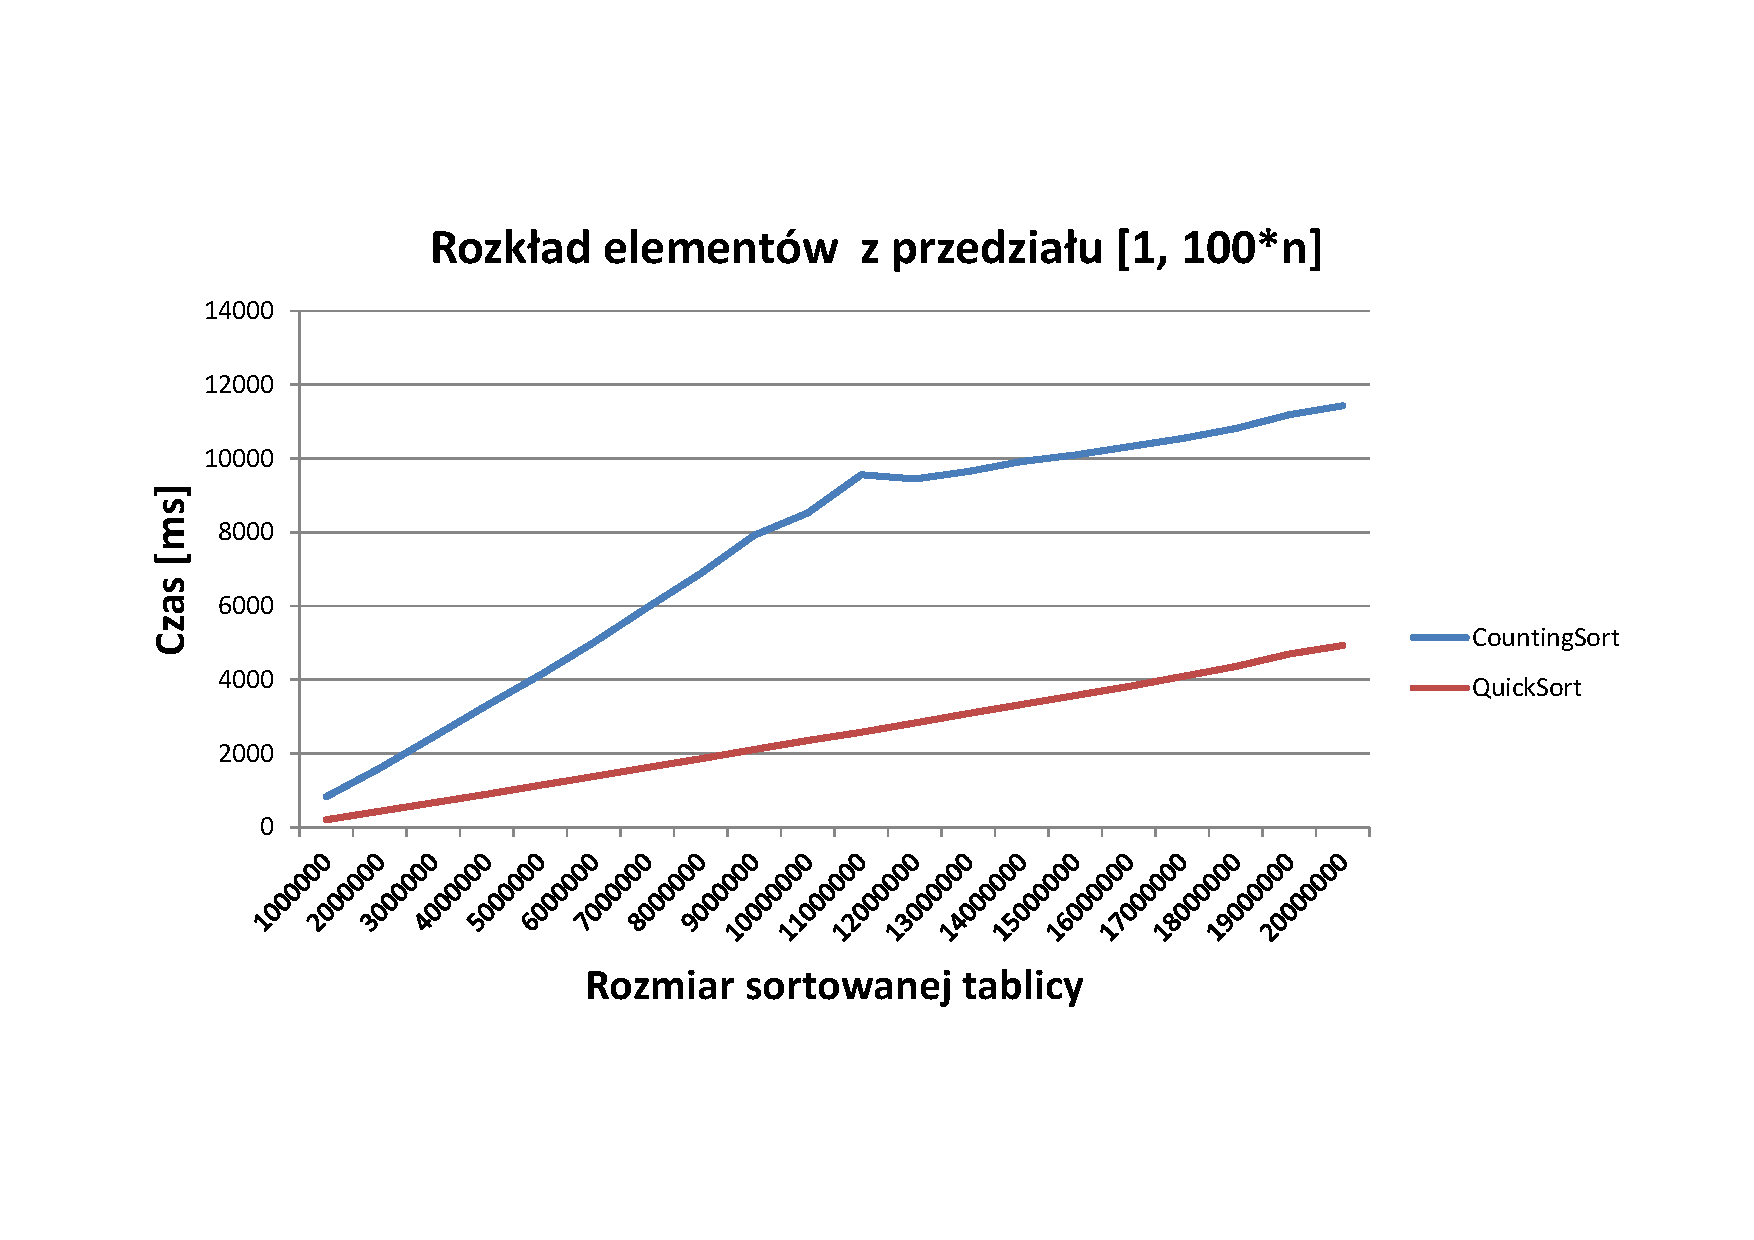
\includegraphics[scale=0.6]{zad4100n.pdf}
		\label{fig:zad4100n}
	\end{center}
\end{minipage}

\subsubsection*{Zrzut ekranu sekcji Diagnostic Tools programu Visual Studio 2015 prezentujący, zużycie pamięci i procesora w trakcie sortowania algorytmami Counting Sort i  Quick Sort, dla rozkładu losowego w przedziale $[1;100n]$.}

\begin{minipage}[H]{\textwidth}
	\begin{center}
		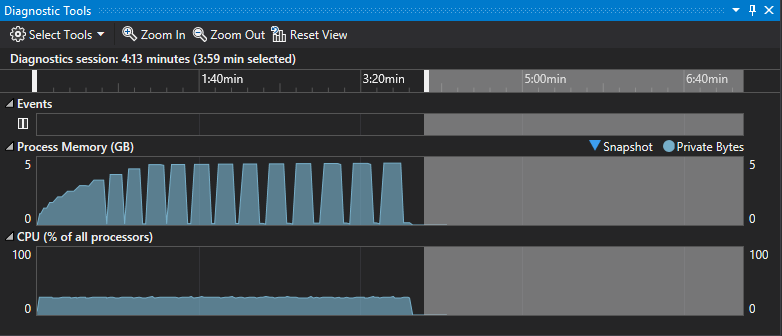
\includegraphics[scale=0.85]{zad4pamiec100n.png}
		\label{fig:zad4pamiec100n}
	\end{center}
\end{minipage}

\subsubsection{Wnioski do przedziału $[1;0,01n]$}


\subsection{Wnioski do badania zależności czasu obliczeń $t$ od liczby sortowanych elementów $n$ dla metod Counting Sort, Quick Sort, przy rozkładzie losowym, gdy wartości elementów mieszczą się w przedziałach  $ [1;0,01n] $,$ [1;100n] $. }
	

	
\end{spacing}
	\newpage
	\tableofcontents
\end{document}


